
\input{english/config.tex}

% Metadata
\title{State registry data access notifications for Estonian eID holders}
\author{Arkadi Statsenko}
\date{2025}
\supervisor{Daniel Würsch\degree{MSc}}% \and Co-Supervisor's name\degree{degree}}
\curriculum{Computer Science Curriculum}
\thesis{Bachelor's Thesis (9 ECTS)}
\keywords{Andmejälgija}


% Here begins the document

\begin{document}

\maketitle

\linespread{1.45} \selectfont

\newpage
\pdfbookmark[1]{\infoname}{info} % Adding the info page among the PDF bookmarks


% English information
\begin{info}
\begin{abstract}
\textit{Andmejälgija} is a protocol developed by Information System Authority (RIA), the purpose of which is to provide a uniform interface for querying Estonian residents' data access logs. There is also an \textit{Andmejälgija} web-view accessible from the state-portal \textit{\href{https://www.eesti.ee}{eesti.ee}}. 

The purpose of this thesis is to create a mobile application that would notify its users of updates in the access logs, letting them know that their data in some state database has been accessed. Implementation choices of different aspects of the solution are also going to be covered together with advantages and disadvantages of each. Additionally, the overview of the existing state databases will be provided, including whether they provide access logs or not.
\end{abstract}

% Visual abstract is not required for all curricula
%\begin{visualAbstract}
%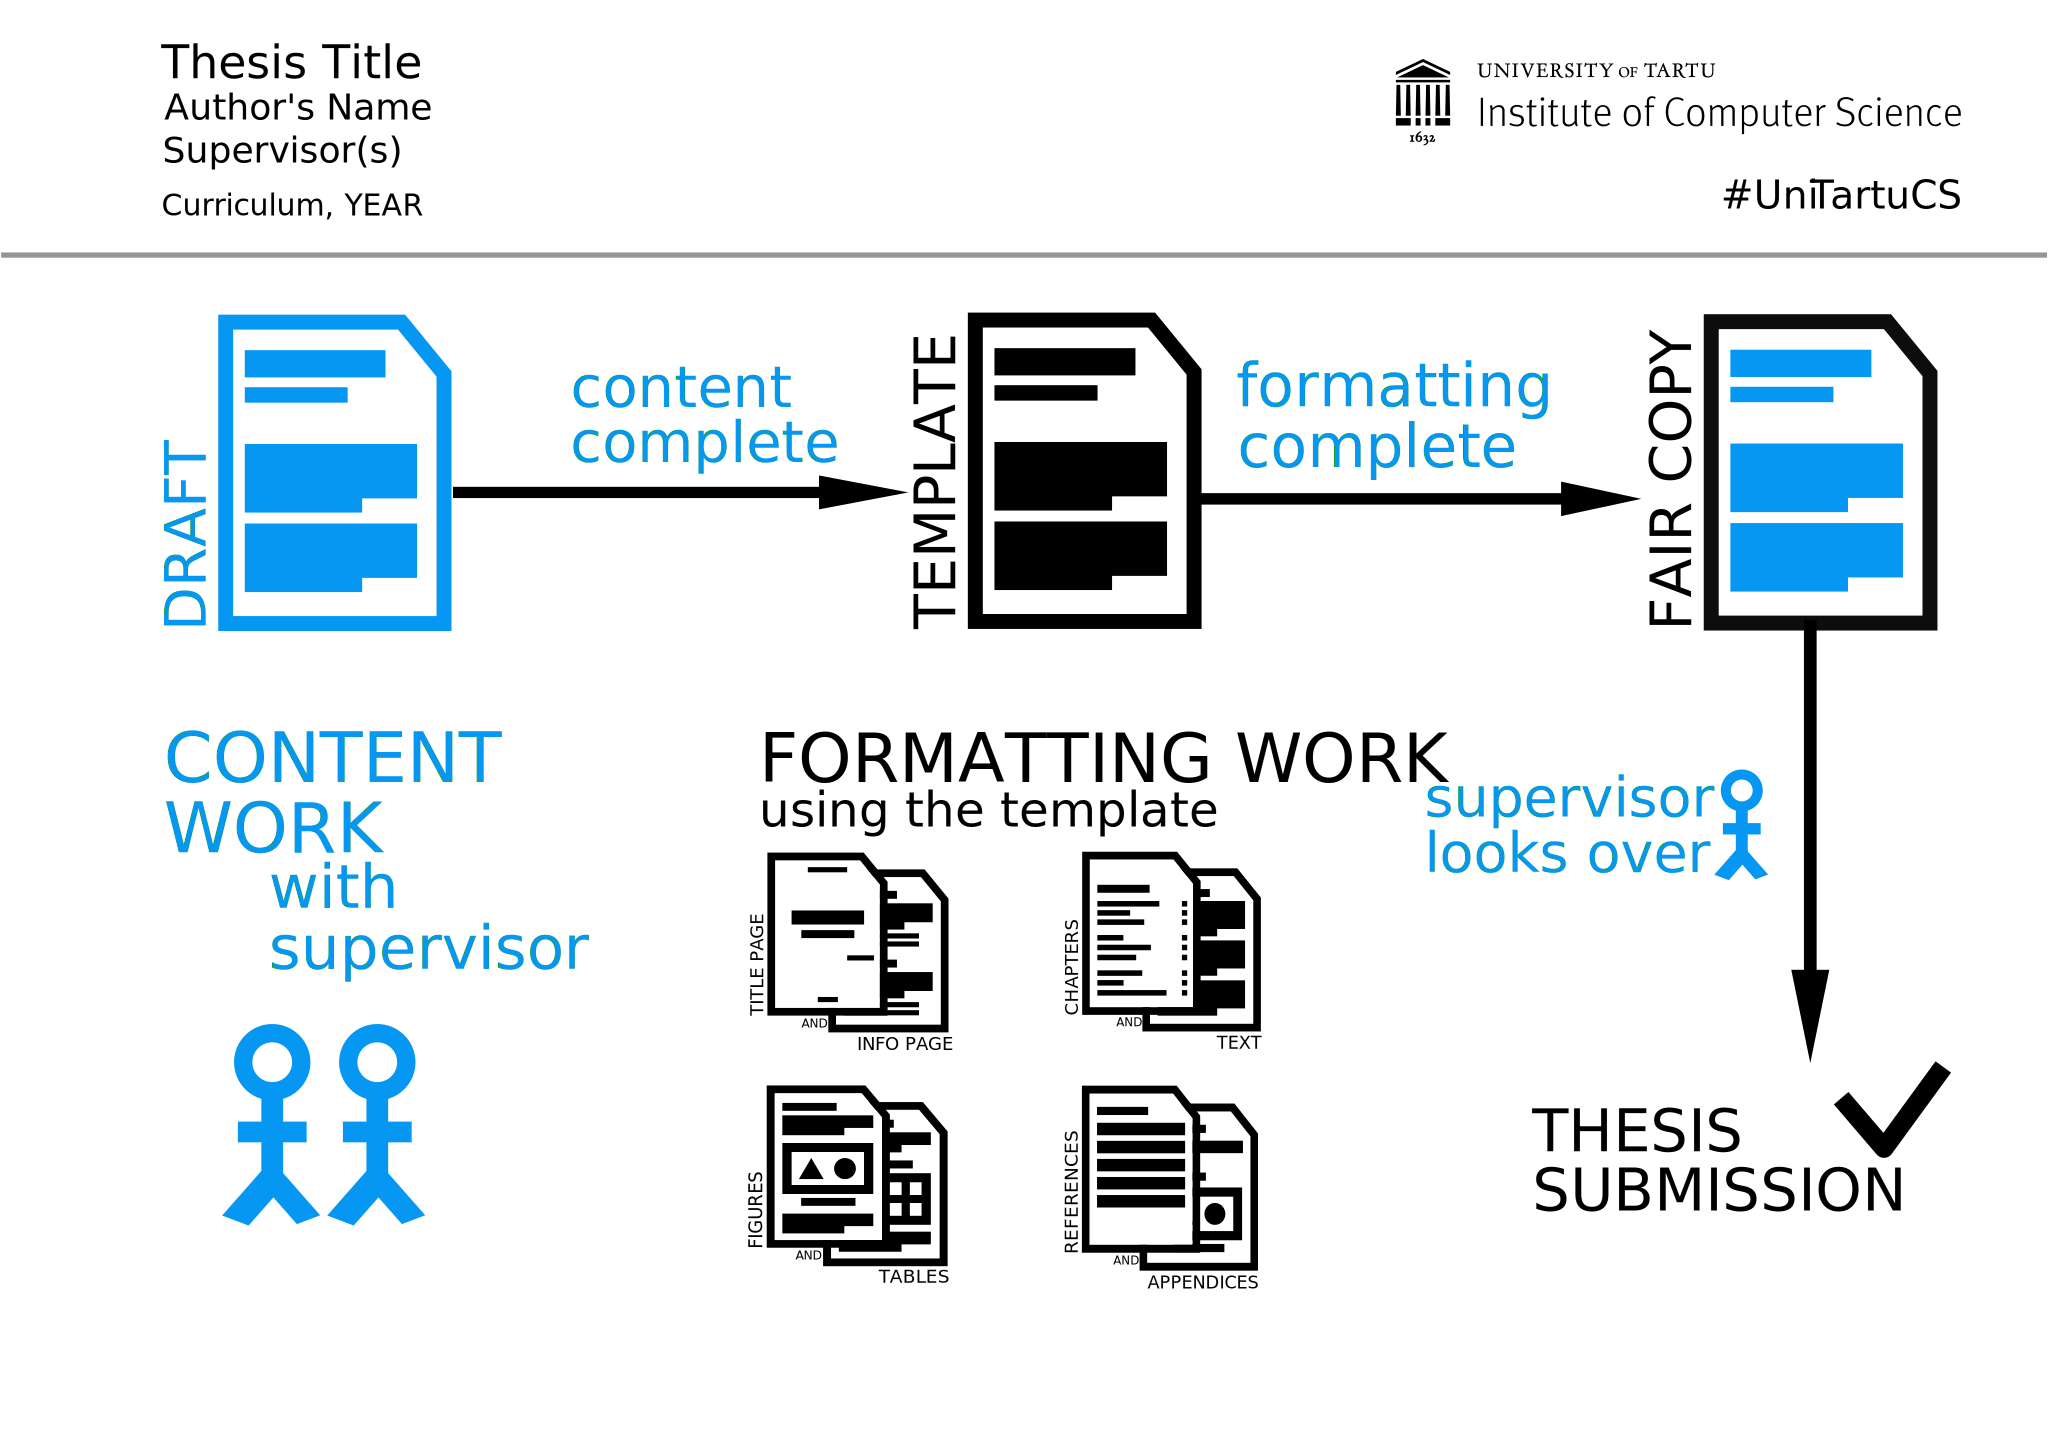
\includegraphics[width=\textwidth]{figures/Figure0-VisualAbstract.png}
%\end{visualAbstract}

% \keywords{}

\cercs{P170 Computer science, numerical analysis, systems, control  }
% Codes can be found at: https://www.etis.ee/Portal/Classifiers/Index/26
% Example: P170 Computer science, numerical analysis, systems, control
% Example: P175 Informatics, systems theory
\end{info}



% Estonian information
\begin{otherInfo}{estonian}{Teavitused riiklike andmekogude andmetele juurdepääsu kohta Eesti eID omanikele}
\begin{abstract}
Käesoleva lõputöö eesmärk on luua rakendus, mis teavitaks kasutajaid juurdepääsulogide uuendustest, andes neile teada, et nende andmeid mõnes riigi andmebaasis on kasutatud. Rakendusel on olnud erinevad rakendusvariandid, mida käsitletakse ka koos igaühe eeliste ja puudustega. Lisaks antakse ülevaade olemasolevatest riiklikest andmebaasidest, sealhulgas sellest, kas nad pakuvad juurdepääsulogisid või mitte.
\end{abstract}

% Visual abstract is not required for all curricula
%\begin{visualAbstract}
%\includegraphics[width=\textwidth]{figures/Figure0-VisualAbstract-est.png}
%\end{visualAbstract}

% \keywords{}

\cercs{T170 Arvutiteadus, arvutusmeetodid, süsteemid, juhtimine (automaatjuhtimisteooria)}
\end{otherInfo}



\tableofcontents

\section{Introduction} \label{Introduction}

In Estonia there are a lot of state databases holding users' data, like Population Registry (\textit{Rahvastikuregister}) and Health Portal (\textit{Terviseportaal}). People's data in these databases is accessed by different parties for the variety of purposes. Usually those are legitimate purposes, like a doctor accessing person's health documents, or people themselves accessing their data in some information systems. However, sometimes the purpose of data access is not clear.

For the purposes of making the process more transparent, the Estonian Information System Authority (RIA) created a special service, Data Tracker (\textit{Andmejälgija}), in 2017, through which users can check which parties have accessed their data \cite{err-population-registry-unauthorized-access}. 

The Data Tracker is a people-oriented service on the state portal \textit{eesti.ee}, which aims to ensure transparency in the processing of personal data in both private and public sectors. The Data Tracker relies on the ability of each state database to store the data processing taking place within itself in the form of logs, in order to later display it to the individual, i.e. the data subject, via the service on \textit{eesti.ee} \cite{aj-github}.

Architecturally, it is a fully distributed system, i.e. the information displayed to the user comes directly from the database that implemented the Data Tracker service. At the user's request, \textit{eesti.ee} makes a query to each of the Data Tracker services and displays the query response without saving it \cite{aj-github}.

The Data Tracker should display to the individual information about data processing taking place locally in the database (activities of officials-employees or automated systems with personal data) as well as an overview of when data has been transferred to a third party (via X-Road to another government agency or private entity) \cite{aj-github}.

The Data Tracker doesn't notify, however, when the data is accessed by someone. In order to learn about the update in the data access logs, the person has to go to the \textit{eesti.ee} web-view and manually query access logs from specific databases. 

The primary objective of this thesis is to solve this problem by creating a mobile phone application that would notify its users about the new data access logs in near-real time. 

Additionally I would like to examine existing state databases processing people's personal data, including whether they provide access logs or not.
\section{\textit{Andmejälgija}} \label{Andmejälgija}

\subsection{The protocol} \label{protocol_desc}

Andmejälgija is a protocol that state databases are responsible for implementing themselves. In order for the database to offer an \textit{Andmejälgija} service, they have to create an X-Road interface according to RIA specification\cite{aj-github-spec}. 

X-Road is a REST-based protocol which is used for secure data exchange between Estonian information systems over the Internet.

The \textit{Andmejälgija} X-Road interface is expected to have the following endpoints:

\textbf{\texttt{findUsage}}

A query searches the data recorder database for usage records that match the constraints given in the input. The output of the query returns all records found\cite{aj-github-spec}.

\textbf{\texttt{usagePeriod}}

The time period for which usage information can be requested\cite{aj-github-spec}.

\textbf{\texttt{heartbeat}}

Requesting the availability status of the tracker's usage information\cite{aj-github-spec}.

The overall architecture of the \textit{Andmejälgija} system is illustrated in Figure~\ref{fig:aj-model}, which shows how state databases interact with the \textit{\href{https://www.eesti.ee}{eesti.ee}} portal through X-Road to provide data access logs to end users.

\begin{figure}[H]
\centering
\includegraphics[width=450px]{english/figures/aj_model.PNG}
\caption{\textit{Andmejälgija} (Data Tracker) system architecture showing the interaction between entities implementing data tracking and \textit{\href{https://www.eesti.ee}{eesti.ee}} Data Tracker view. The data exchange happens via X-Road\cite{aj-github}.}
\label{fig:aj-model}
\end{figure}

\subsection{Usage}
There are several ways for end-users to access their Data Tracker data. State portal \textit{\href{https://www.eesti.ee}{eesti.ee}} provides a web-view for \textit{Andmejälgija} where end users can access their data access logs. Recently, RIA have also published a mobile application for \textit{\href{https://www.eesti.ee}{eesti.ee}}, that also features a view of data access logs. 

Another way to access Data tracker data is through Estonian Population Registry, although, is seems to be Population Registry specific as it doesn't provide access logs from other databases



\subsection{Adoption}
The current adoption of \textit{Andmejälgija} has some noticeable issues. Very often it is not at all clear why your data have been accessed, at least from the first glance. Explanation messages are vague and confusing, often being similar to ``data access by personal code'', making it difficult to understand the reason behind the data access, even if it was you who accessed it.

There is even an information sheet with recommendations for services implementing the \textit{Andmejälgija} protocol, and it states that providing poor quality explanations for data access is a bad practice\cite{ria-andmejalgija-recommendations}. The good and poor examples of data access descriptions are shown in Table~\ref{tab:example-good} and Table~\ref{tab:example-bad}.

\textbf{Good practice example:}

\begin{table}[H]
\centering
\begin{tabular}{|p{3cm}|p{6cm}|p{4cm}|}
\hline
\textbf{Data Processing Time} & \textbf{Activity} & \textbf{Party Receiving Personal Data} \\
\hline
13.01.2015 10:20:27 & Prescription viewed by doctor; prescription number 1018472350 & Doctor Viktor Pihlakas \\
\hline
19.01.2018 10:58:23 & Individual query for valid driver's licenses through state portal \textit{\href{https://www.eesti.ee}{eesti.ee}} & Jaan Kask 32405023456 \\
\hline
\end{tabular}
\caption{Example of good data access descriptions\cite{ria-andmejalgija-recommendations}}
\label{tab:example-good}
\end{table}

\textbf{Bad practice example:}

\begin{table}[H]
\centering
\begin{tabular}{|p{3cm}|p{6cm}|p{4cm}|}
\hline
\textbf{Data Processing Time} & \textbf{Activity} & \textbf{Party Receiving Personal Data} \\
\hline
13.01.2015 10:20:27 & PERSONAL DATA BY PERSONAL CODE & INSTITUTION X \\
\hline
19.01.2018 10:58:23 & INDIVIDUAL EXTENDED INFO QUERY BY PERSONAL CODE & FOUNDATION Y \\
\hline
\end{tabular}
\caption{Example of poor data access descriptions\cite{ria-andmejalgija-recommendations}}
\label{tab:example-bad}
\end{table}

Apparently, the advice is often ignored, as many institutions tend to follow the bad example in practice. The thesis author's Data Tracker view is flooded with entries containing poor quality descriptions like those shown in Table~\ref{tab:author-data-tracker}.

\begin{table}[H]
\centering
\begin{tabular}{|p{2.5cm}|p{5cm}|p{3cm}|p{3.5cm}|}
\hline
\textbf{Date \& Time} & \textbf{Institution} & \textbf{Database} & \textbf{Activity} \\
\hline
02.08.2025 11:15 & Health and Welfare Information Systems Centre & Population Registry & INDIVIDUAL EXTENDED INFO QUERY BY PERSONAL CODE \\
\hline
01.08.2025 22:37 & Health and Welfare Information Systems Centre & Population Registry & INDIVIDUAL NAME RETRIEVAL BASED ON PERSONAL CODE \\
\hline
01.08.2025 20:23 & Education and Youth Board & Population Registry & PERSONAL DATA BY PERSONAL CODE \\
\hline
\end{tabular}
\caption{Extract from author's Data Tracker view demonstrating poor quality descriptions}
\label{tab:author-data-tracker}
\end{table}

Furthermore, currently there is no law requiring institutions to implement the \textit{Andmejälgija} protocol, meaning that its use is essentially voluntary. This may change in the future, however, as the current coalition government formed by the Estonian Reform Party and Eesti 200 has promised to make the use of \textit{Andmejälgija} compulsory according to their coalition agreement\cite{coalition-agreement-2025-2027}.

In the following chapter, different state databases and their implementations of \textit{Andmejälgija} will be covered, including whether they implement the protocol at all.
\section{Overview of state databases} \label{Overview of state databases}

\subsection{Databases implementing Andmejälgija}

\begin{itemize}
    \item{Digiregistratuur}
    \item{Elamislubade ja töölubade register}
    \item{Kinnistusraamat}
    \item{Kutseregister}
    \item{Maksukohustuslaste register}
    
    \item{Politsei taktikalise juhtimise andmekogu}
    \item{Põllumajandusloomade register}
    \item{Põllumajandustoetuste ja põllumassiivide register}
    \item{Rahvastikuregister}
    \item{Retseptikeskus}
    \item{Sotsiaalkaitse infosusteem}
    \item{Sotsiaalteenuste ja toetuste register}
    \item{Tööinspektsiooni tooelu infosusteem}
    \item{Töötuskindlustuse andmekogu}
\end{itemize}
POLIS Information System, while in the list of the Andmejälgija view on Eesti.ee, actually doesn't show any entries even if they should be there.

\subsection{Databases providing other form of data access tracking}
\begin{itemize}
    \item{E-toimik}: provides it's own web-view for displaying requests made about you.
    \includegraphics[width=450px]{english/figures/e-toimik.png}
\end{itemize}




\subsection{Databases not providing any kind of data access tracking}
\begin{itemize}
    \item{Schengen Information System}
    \item{Piirikontrolli andmekogu (PIKO)}
    \item{Infosusteem POLIS}
\end{itemize}

\section{Implementation}

\subsection{Description}

The main objective of this thesis has been to develop a solution that would notify the user about new entries in Data Tracker.

\subsection{Discussion of implementation choice}
There is a number of possible ways to develop such a solution. In this section I will discuss different implementation options, the advantages and disadvantages of each, as well as why I eventually decided to settle on creating an Android application.

\subsubsection{X-Road service}
Andmejälgija specifications requires databases to implement an X-Road interface, as described in \ref{protocol_desc}, so one option would be to create an X-Road service that would query Andmejälgija data over X-Road. The main advantage of this approach would be the freedom on how to notify the users of changes to the access logs. The service could support various channels of communication, including instant messenger bots, e-mail and others. The list of requirements in order to operate such a service is daunting, however. 

\begin{itemize}
    \item {In order to join X-Road, legal entity is needed}
    \item {Permission has to be requested from every X-Road service you want to query data from}
    \item {As part of X-Road network, you need to operate a Security Server. It can be self-hosted anywhere for testing, but for production you need to have a Hardware Security Module (HSM), in order to be compliant with eIDAS requirements. HSM costs typically around 10000€. Renting a production ready Security server from Telia costs 210€ per month \footnote{\url{https://www.telia.ee/ari/it-teenused/serverid-ja-pilv/x-tee-turvaserver/}}}
\end{itemize}

Satisfying this criteria is difficult and expensive. Additionally, even if I succeeded, people would have to consent and entrust me with their data in order to be able to use the solution.

\subsubsection{Standalone approach}
This approach uses Eesti.ee session for accessing Andmejälgija data. Once the user is logged in on eesti.ee state portal, certain internal API endpoints become available. Namely GET https://www.eesti.ee/andmejalgija/api/v1/usages endpoint can be used to query Andmejälgija data. The endpoint requires a parameter dataSystemCodes with which specific databases can be specified. For example GET request /usages?dataSystemCodes=digiregistratuur\&dataSystemCodes=rahvastikuregister would request access logs from Digiregistratuur and Rahvastikuregister.

The main advantage of this approach is the abscence of all disadvantages of the X-Road approach: there is no need for any kind of bureaucracy and the solution could be an open-source project, available for anybody to compile and use. There arises a problem, however. What about the notification part? Do I expect users to set everything up on their hardware, including relevant communication channels? That would narrow down the project's user base to technical people knowing how to self-host, and having a server.

That's why I thought that creating a mobile app would be the most optimal approach. The app would keep the eesti.ee session alive and poll the Data Tracker API. This approach would combine the ease of setting up and use with solution remaining standalone, without a central server.

\subsection{Development}

First of all I had to determine how feasible and reliable the standalone approach would be, especially as I was dealing with user-facing service that I would have to effectively reverse-engineer. The main challenge was to keep the session alive for as long as possible,

The eesti.ee session is established using one of strong authentication methods via TARA authentication service. Once the user is authenticated using ID-card, Mobile-ID, Smart-ID, or eID solution of another EU country, a JWT token is issued, valid for 30 minutes. Once the user is authenticated, certain internal API endpoints become available, including those for refreshing JWT token and getting Data Tracker access logs. The JWT refresh endpoint returns Set-Cookie headers that include an updated JWTTOKEN on success, with updated expiration date (30 minutes from the moment of extention).

In order to test whether the session could be kept alive indefinitely I used Tab Reloader extention for Firefox by James Fray \footnote{\url{https://addons.mozilla.org/en-US/firefox/addon/tab-reloader/}}. Using the browser extention I set up browser to auto reload tab with JWT token refresh endpoint. After 8 hours of experiment I deemed it a success.

Next step was the development of Android application. I have chosen to develop it using Kotlin programming language due to it being a new standard for developing Android apps as well as it having more expressive syntax and promising faster development speed.

The app is compatible with all Android versions starting from Android 8.1, meaning that it would work on approximately 96.4\% of Android devices according to Android Studio API version distribution chart.

\includegraphics[width=450px]{english/figures/Screenshot from 2025-08-04 19-37-39.png}

The software is open-source, licenced under MIT licence.

At the moment the application support is limited to Android 8.1 and higher. While support for IOS and other platforms is not planned due to limited development time and resources, the author would like to encourage anybody who would deem this solution useful to port it to platforms other than Android.

\subsubsection{Authentication}
In order to get access to eesti.ee internal APIs, the used needs to be authenticated via TARA. An initial plan has been to reverse engineer the authentication flow and authenticate the user by sending raw http requests and sending back responses. This approach, however would be fragile and require substantial engineering effort to develop and maintain.

Instead, I decided to use Android WebView for authentication as a more reliable and convenient approach for both the user and the developer. By leveraging WebView, the app can present the official TARA login page directly to the user, allowing them to authenticate using their preferred method (ID-card, Mobile-ID, Smart-ID, or eID of another EU country). This approach significantly reduces the risk of breaking changes due to updates on the eesti.ee or TARA platforms. Once the user is authenticated, the app can access the necessary session cookies and JWT token to interact with the internal APIs.

\subsubsection{Interacting with eesti.ee internal APIs}
For interacting with eesti.ee internal API I used OkHttp library by Square, Inc. \footnote{\url{https://square.github.io/okhttp/}}. I have used the following API endpoints:

\begin{itemize}
    \item \textbf{GET} \texttt{https://www.eesti.ee/timur/jwt/extend-jwt-session}
    
    An endpoint for extending JWT session.
    
    \item \textbf{GET} \texttt{https://www.eesti.ee/andmejalgija/api/v1/usages}
    
    An endpoint for querying Data Tracker access logs.
    
    Query parameters:
    \begin{itemize}
        \item \texttt{dataSystemCodes}: The name of the information system the access logs are queried from.
    \end{itemize}
    
    \samepage
    Response body format (JSON):
    \begin{small}
    \begin{verbatim}
{
  "findUsageResponses": [
    {
      "logTime": "2025-08-03T22:40:47",
      "receiver": "Tervise ja Heaolu Infosüsteemide Keskus",
      "infoSystemCode": "rahvastikuregister",
      "action": "ISIKU NIME VÄLJASTAMINE ISIKUKOODI PÕHJAL"
    },
    ...
  ]
}
    \end{verbatim}
    \end{small}
    
    Response fields:
    \begin{itemize}
        \item \texttt{logTime}: Timestamp of the data access event in ISO 8601 format
        \item \texttt{receiver}: Registry code of the entity that accessed the data
        \item \texttt{infoSystemCode}: Code identifying the information system
        \item \texttt{action}: Description of the action performed (in Estonian)
    \end{itemize}
\end{itemize}

Both endpoints require a valid JWT token in order to succeed. WebView's CookieManager serves as a single source of truth in this application, where all cookies are loaded from for making requests and written to on responses.

\subsubsection{Keeping the session alive}
The API requests are authenticated using JWT token cookie, the lifetime of which is 30 minutes. This means that the app has to either run a continuous foreground service or be waken up every once in a while in order to request an updated JWT token and send requests to Data Tracker.

On Android there are several ways to accomplish this, although it's worth mentioning that Android is very restrictive regarding background tasks and battery usage. I have tried several approaches and will describe my experience with them in the context of developing this app.

\paragraph{WorkManager}
According to Android documentation WorkManager is the recommended solution for persistent work, Work is persistent when it remains scheduled through app restarts and system reboots. This seemed to describe my use case very well, so that was the first approach that I have tried.

Work is defined in WorkManager using a WorkRequest. There are several WorkRequest types available, including PeriodicWorkRequest and OneTimeWorkRequest.

Using PeriodicWorkRequest, it is possible to schedule periodic tasks. The important limitation here is that it is not possible to schedule a task to execute more frequently than every 15 minutes. While this may sound appropriate for the use case of having to renew the session at least every 30 minutes, in reality things look differently.

During development, I discovered a critical difference between session handling in web browsers versus HTTP client libraries. While the browser-based testing with Tab Reloader successfully maintained the session by refreshing the JWT token every 15 minutes, the same approach using OkHttp in the Android application failed to keep the session alive .

The exact cause of this discrepancy remains unclear. It appears that the eesti.ee session management system expects more frequent interaction or handles cookie management differently when requests originate from HTTP client libraries compared to full web browsers. And indeed, with shorter intervals of 5 minutes the session stays alive. This behavioral difference rendered the PeriodicWorkRequest approach with 15-minute intervals unsuitable for maintaining persistent sessions in the application context.

While OneTimeWorkRequest is meant for one time tasks, it is possible to chain them by having each one-time work create another one-time work at the end of it's lifespan.This approach allows to set custom intervals shorter than 15 minutes, curcumventing the limitation imposed by PeriodicWorkRequest.

While OneTimeWorkRequest may sound like a good solution, WorkManager itself appeared to be rather unreliable for my use case after some testing. The core reason behind limitations to follow is that tasks scheduled by WorkManager are managed by the system and may be deffered if deemed needed by the Android system, for example in the low battery scenario, or even in other scenarios depending on the aggressivenes of the Android variant in regards to the restrictions imposed on the behaviour of the apps.

\paragraph{Foreground Service}
Foreground service is one of the most reliable types of tasks the application can schedule. As opposed to background services, foreground services are considered to be of higher priority to the system and thus are not candidates for being killed when the system is low on memory or the phone is low on battery.

An important limitation has been introduced in the latest Android updates though. More specifically, starting from Android 15, he system places restrictions on how long certain foreground services are allowed to run while your app is in the background. Currently, this restriction only applies to dataSync and mediaProcessing foreground service type foreground services.

The most appropriate foreground service type for my use case is dataSync, meaning that it falls under the 6 hour restriction. While it should be possible to choose an arbitrary foreground service type regardless of the type of an actual task, doing so is not the cleanest approach, especially considering the existance of better alternatives. Furthermore, doing so may also impact the app being accepted into Google Play Store.

\paragraph{AlarmManager + dataSync foreground service}

After evaluating the limitations of WorkManager and the restrictions on foreground services, I ultimately settled on a hybrid approach combining AlarmManager with a dataSync foreground service. AlarmManager is a system service that allows scheduling operations to be executed at specific times, even if the app is not running. By using AlarmManager to trigger the app at regular intervals (e.g., every 5 minutes), I ensure that the session renewal and data polling tasks are reliably executed.

When the alarm fires, the app starts a short-lived dataSync foreground service to perform the necessary network operations: refreshing the JWT token and querying the Data Tracker API. This approach leverages the reliability of foreground services for critical tasks while minimizing battery usage by only running the service when needed. AlarmManager itself is not subject to aggressive background restrictions and can wake the app even in Doze mode, making it suitable for periodic tasks.

This solution proved to be robust and reliable across different Android versions and device manufacturers. Both AlarmManager and foreground services are extremely reliable even on low battery, ensuring that the session remains alive and notifications are delivered promptly to the user.






\subsection{User guide}
\subsection{Software distribution}
\subsection{Known problems}

%\input{sections/2-formatting}
%\input{sections/3-textCreation}
\section{Conclusion} \label{Conclusion}
The prime objective of this thesis, which is to create a mobile phone app, Data Access Notifier, has been achieved. Even though it has known limitations, it still provides valuable functionality in terms of providing notifications about data access that could have been missed otherwise, especially considering that, as observed in section \ref{observations}, sometimes old logs are delivered with delay of several months.

\section{Discussion}

While an initial solution has been successfully implemented, there remains considerable scope for further development and enhancement.

\subsection{Future Development Opportunities}

Several potential approaches could address the current 12-hour session limitation by exploring alternative authentication flows and API endpoints. One avenue for investigation would involve reverse-engineering the official eesti.ee Android application to analyze its authentication mechanisms, for example by decompiling it's APK and studying the resulting source code. The application is known to support biometric authentication with PIN code fallback functionality. Through proper reverse engineering and reimplementation of these authentication flows, it may be theoretically possible to automate PIN code resubmission and maintain indefinite session validity.

However, such an approach would constitute a substantial undertaking that could warrant a separate research project. Additionally, this method would likely introduce significantly greater implementation complexity compared to the current solution, potentially making it more fragile and maintenance-intensive.

\subsection{Optimal Solution}

The most effective solution would be for RIA (Information System Authority) to implement equivalent functionality directly within the eesti.ee platform. Such an official implementation would be relatively straightforward to develop and would provide superior reliability and future-proofing compared to any third-party solution, including the one presented in this thesis.
\clearpage
\printbibliography[heading=bibintoc]
\section{Glossary}

\subsection{Estonian Government and Technology Terms}

\begin{description}
    \item[\textit{Andmejälgija}] Data Tracker - Protocol developed by RIA for tracking personal data access across state databases.
    
    \item[\textit{eesti.ee}] Official Estonian state portal providing access to various government e-services.
    
    \item[\textit{TARA}] Trusted Authentication and Authorization service - Estonian government service that handles initial user authentication using strong authentication methods (ID-card, Mobile-ID, Smart-ID, EU eID).
    
    \item[\textit{GovSSO}] Government Single Sign-On service - manages session state and enables users to access multiple Estonian government e-services with a single authentication. Works in conjunction with TARA to provide seamless access across government platforms.
    
    \item[\textit{Digiregistratuur}] Digital patient registry system in Estonia.
    
    \item[\textit{Rahvastikuregister}] Estonian Population Register containing basic demographic information.
    
    \item[\textit{E-File}] The E-File is a central information system that provides an overview of the different phases of criminal, civil, administrative and misdemeanour proceedings, procedural acts and court adjudications to all the parties involved, including the citizen and their representatives\cite{e-file-rik}. Includes the data access tracker for Criminal Records Database. 
    
    \item[RIA] \textit{Riigi Infosüsteemi Amet} - Information System Authority, the Estonian government agency responsible for information systems.
    
    \item[X-Road] Estonian data exchange platform that enables secure data exchange between information systems.
    
    \item[eIDAS] Electronic Identification, Authentication and Trust Services - EU regulation for electronic identification and trust services.
\end{description}

\subsection{Android Development Terms}

\begin{description}
    \item[AlarmManager] Android system service for scheduling operations to be executed at specific times.
    
    \item[WorkManager] Android Jetpack library for deferrable, guaranteed background work. Uses JobScheduler for API 23+, and AlarmManager + BroadcastReceiver for API 14-22. Automatically chooses the best execution method based on Android version and system constraints \cite{android-workmanager}.
    
    \item[Foreground Service] Android service that runs in the background but displays a persistent notification to the user, making the user aware of the ongoing operation. Despite running in the background, it's called "foreground" because it maintains user visibility through the notification.
    
    \item[Background Service] Android service that runs without user awareness and without displaying notifications. These services are heavily restricted by the system to preserve battery life and system performance.
    
    \item[WebView] Android component that displays web content within an application.
    
    \item[OkHttp] HTTP client library for Android and Java applications.
    
    \item[Proto Data Store] Android library for storing typed objects using protocol buffers.
    
    \item[Doze Mode] Android power-saving feature that defers background CPU and network activity for applications.
    
    \item[APK] Android Package - file format used to distribute and install applications on Android.
    
    \item[JWT] JSON Web Token - method for transmitting information between parties as a signed JSON object.
\end{description}

%\input{sections/10-appendices}
\section*{License} \label{license} \addcontentsline{toc}{section}{License}



\end{document}



